
\subsection{katz-eig}\label{sec:param:katzeig}

There are two parameters to \textit{katz-eig}: $\beta$, the link diminishing factor and $K$ specifying the $K$-rank approximation. $\beta$ is a continous value satisfying $0 < \beta \leq \frac{1}{\|A_{train}\|_2}$. If $\beta = 0$ then the algorithm will only output 0 and if $\beta > \frac{1}{\|A_{train}\|_2}$ the iterations will not converge. $K > 0$ is a discrete value.

What follows is plots over both of the parameters $K$ and $\beta$.

\begin{figure}[h!]
\centering
\begin{minipage}{.5\textwidth}
    \centering
    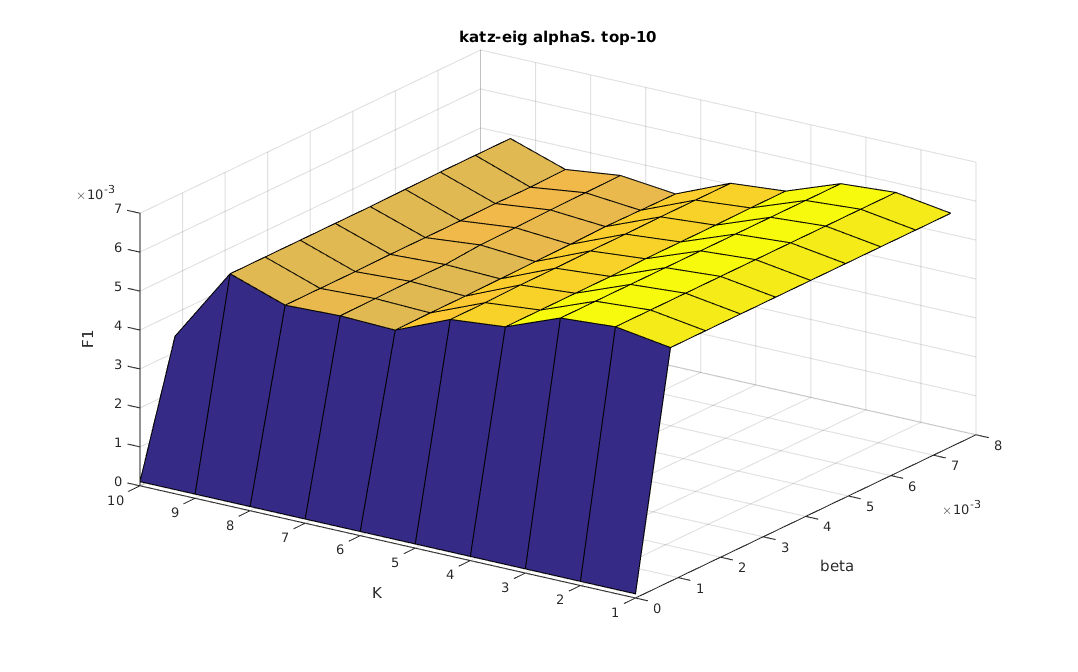
\includegraphics[width=\linewidth]{fig/katzeig_beta_k/alphaS_katzeig.png}
    \captionof{figure}{\textit{alphaS}}
\end{minipage}%
\begin{minipage}{.5\textwidth}
    \centering
    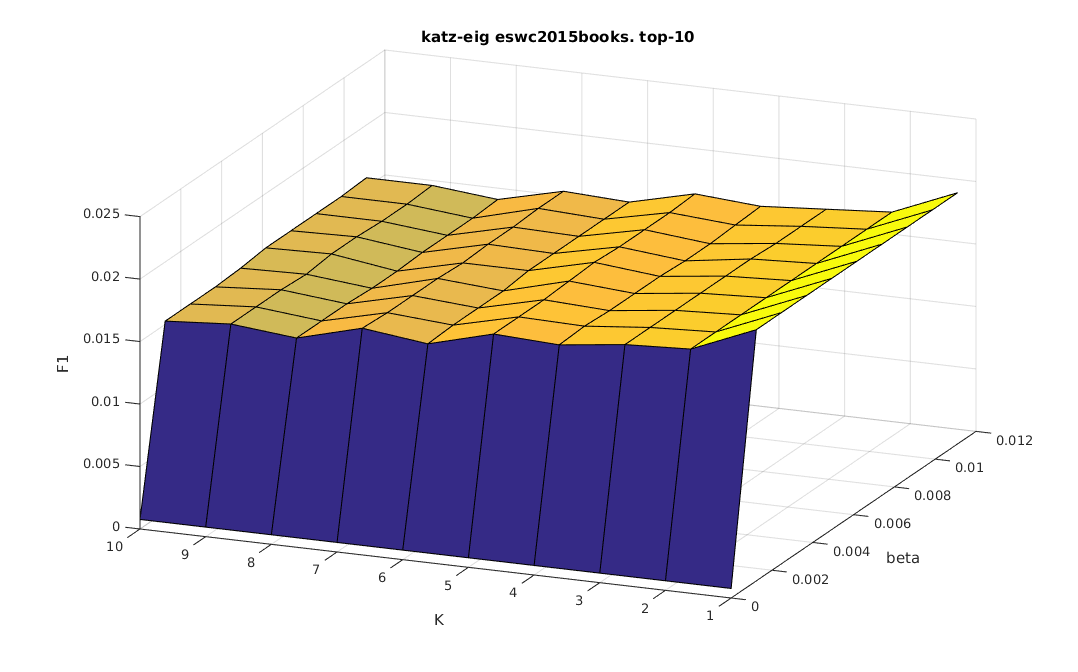
\includegraphics[width=\linewidth]{fig/katzeig_beta_k/eswc2015books_katzeig.png}
    \captionof{figure}{\textit{eswc2015books}}
\end{minipage}
\end{figure}

\begin{figure}[h!]
\centering
\begin{minipage}{.5\textwidth}
    \centering
    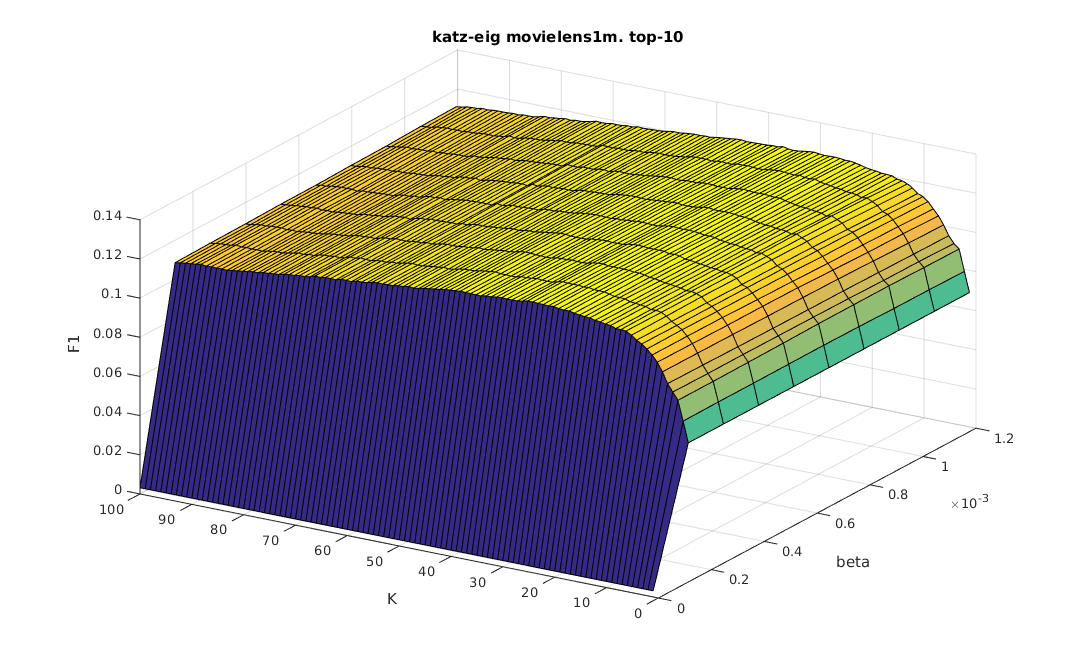
\includegraphics[width=\linewidth]{fig/katzeig_beta_k/movielens_katzeig.png}
    \captionof{figure}{\textit{movielens1m}}
\end{minipage}%
\begin{minipage}{.5\textwidth}
    \centering
    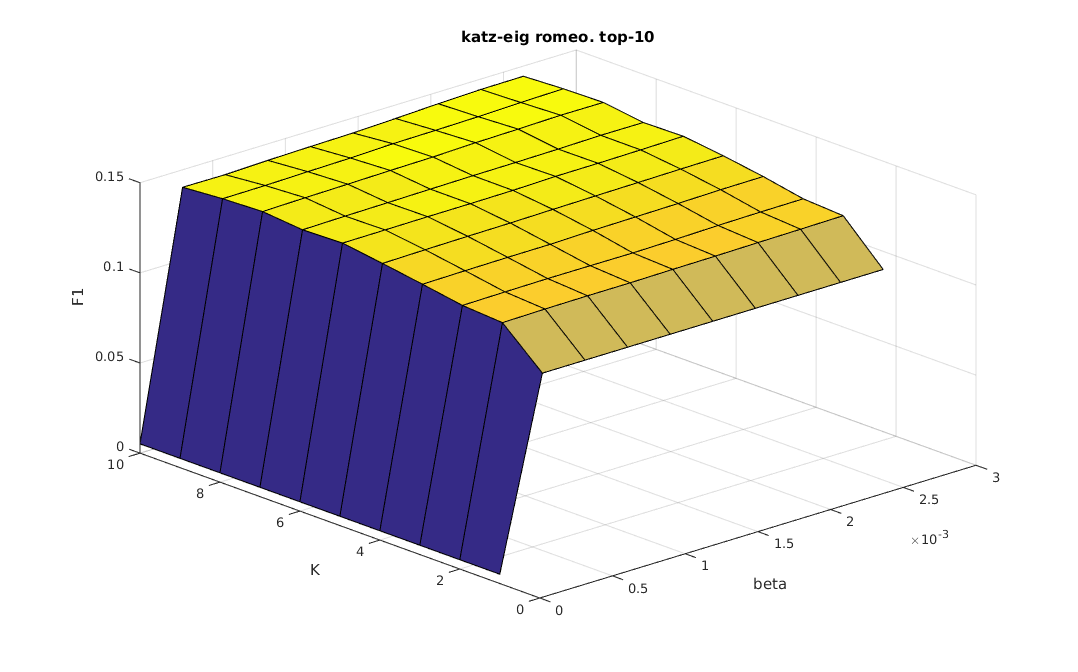
\includegraphics[width=\linewidth]{fig/katzeig_beta_k/romeo_katzeig.png}
    \captionof{figure}{\textit{romeo}}
\end{minipage}
\end{figure}


It seems like $beta$ doesn't have a very big impact on the function value. Some plots with a fixed $K$ follows to better see differences.

The range examined is $0 < \beta \leq \beta_{max} = \frac{1}{\|A_{train}\|_2}$ with a $K$ optimized as described in \sectionref{sec:opt_params}.

\FloatBarrier

\begin{figure}[h!]
\centering
\begin{minipage}{.5\textwidth}
    \centering
    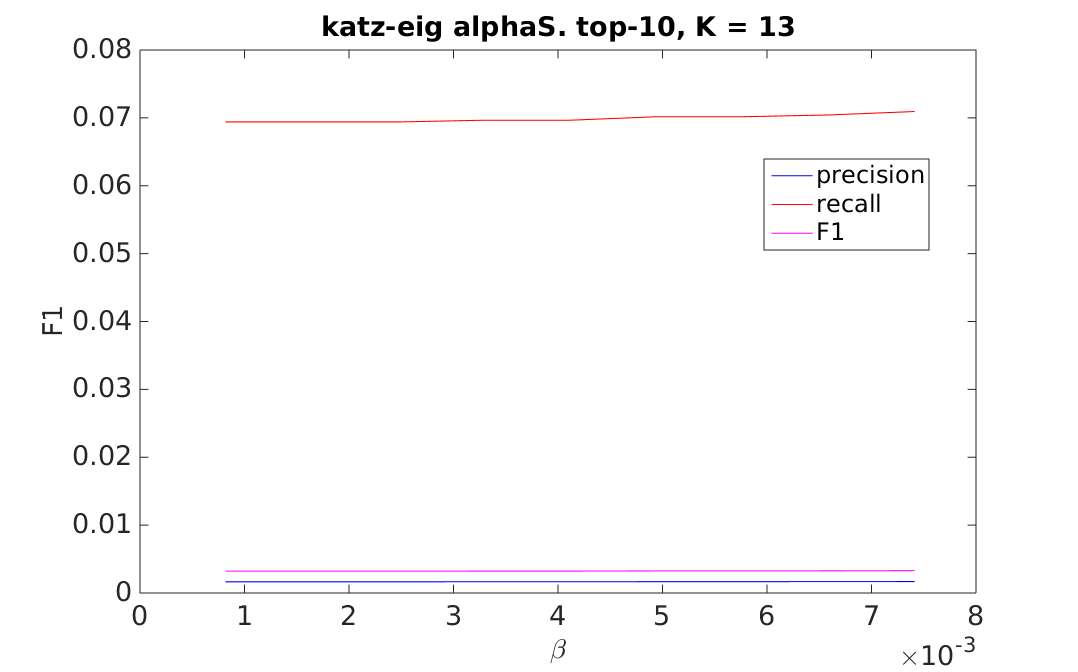
\includegraphics[width=\linewidth]{fig/katzeig_beta/alphaS_katzeig_beta.png}
    \captionof{figure}{\textit{alphaS}.
        $\beta_{max}$ is the best value with a $1.9\%$ diff between the minimum and the maximum \textit{F1} value.}
\end{minipage}%
\begin{minipage}{.5\textwidth}
    \centering
    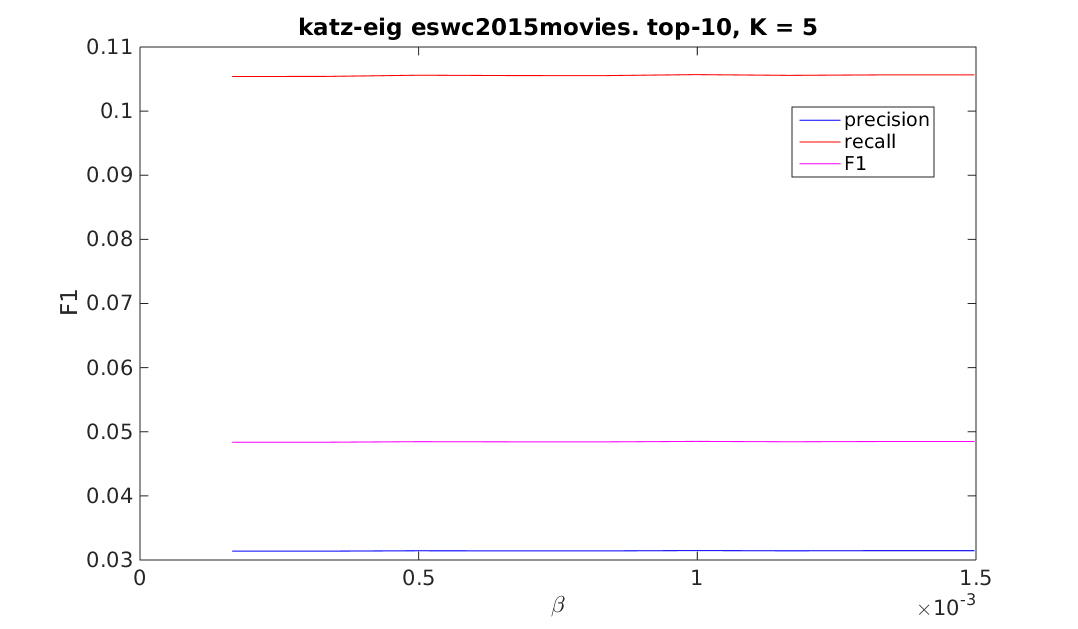
\includegraphics[width=\linewidth]{fig/katzeig_beta/eswc2015movies_katzeig_beta.png}
    \captionof{figure}{\textit{eswc2015movies}.
        $\beta_{max}$ is not the best value with a $0.3\%$ diff between the minimum and the maximum \textit{F1} value.}
\end{minipage}
\end{figure}

\begin{figure}[h!]
\centering
\begin{minipage}{.5\textwidth}
    \centering
    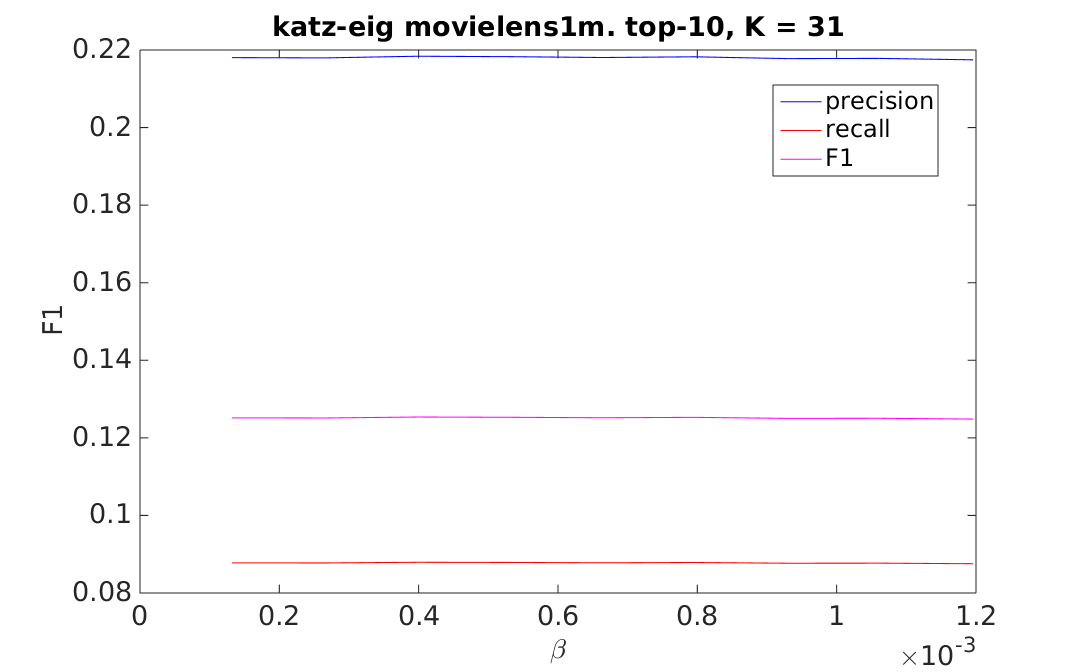
\includegraphics[width=\linewidth]{fig/katzeig_beta/movielens_katzeig_beta.png}
    \captionof{figure}{\textit{movielens1m}.
        $\beta_{max}$ is not the best value with a $0.41\%$ diff between the minimum and the maximum \textit{F1} value.}
\end{minipage}%
\begin{minipage}{.5\textwidth}
    \centering
    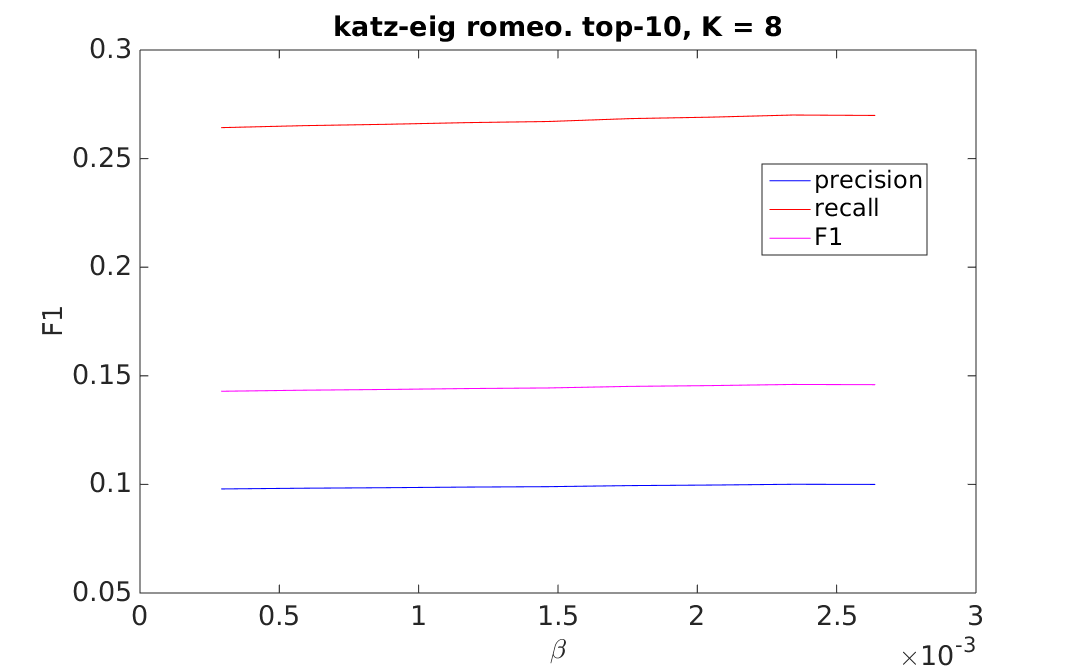
\includegraphics[width=\linewidth]{fig/katzeig_beta/romeo_katzeig_beta.png}
    \captionof{figure}{\textit{movielens1m}.
        $\beta_{max}$ is not the best value with a $2.09\%$ diff between the minimum and the maximum \textit{F1} value.}
\end{minipage}
\end{figure}

\FloatBarrier

The difference between the optimal $\beta$ and an arbitrary selected $\beta$ isn't very large. Even smaller is the difference between the optimal $\beta$ and $\beta_{max}$.  \Tableref{tab:katzeig_beta} is a summary of the evaluated values.

\begin{table}[h!]
    \centering
    \begin{tabular}{| c | r | r | r | r | l |}
        \hline
        \textbf{dataset}        & \textbf{diff between $\beta_{opt}$ and $\beta_{max}$ }    & \textbf{diff between $f_{min}$ and $f_{max}$} \\ \hline

        \textit{alphaS}         & 0~\%      & 2.0~\%    \\ \hline
        \textit{eswc2015books}  & 0~\%      & 0\%       \\ \hline
        \textit{eswc2015movies} & 0.039~\%  & 0.28~\%   \\ \hline
        \textit{movielens1m}    & 0.41~\%   & 0.41~\%   \\ \hline
        \textit{romeo}          & 0.072~\%  & 2.1~\%    \\ \hline


    \end{tabular}
    \caption{A summary of evaluating different $\beta$. $\beta_{max} = \frac{1}{\|A_{train}\|_2}$ is the maximally examined $\beta$ and $\beta_{opt}$ is the optimal $\beta$ found in the range $0 < \beta \leq \beta_{max}$. $K$ is individually optimized for the different datasets. $f_{min}$ and $f_{max}$ are the minimal and maximal \textit{F1} values obtained.}
    \label{tab:katzeig_beta}
\end{table}

\FloatBarrier

\newpage


The $K$-rank approximation represents different available models for \textit{katz-eig}. The following plots show different values of $K$. $\beta = \frac{1}{\|A_{train}\|}_2$ for all datasets as the difference between it and the optimal value is neglible. $K_{m}$ is the value of $K$ which gives the best \textit{F-measure} for each dataset.

\FloatBarrier

\begin{figure}[h!]
\centering
\begin{minipage}{.5\textwidth}
    \centering
    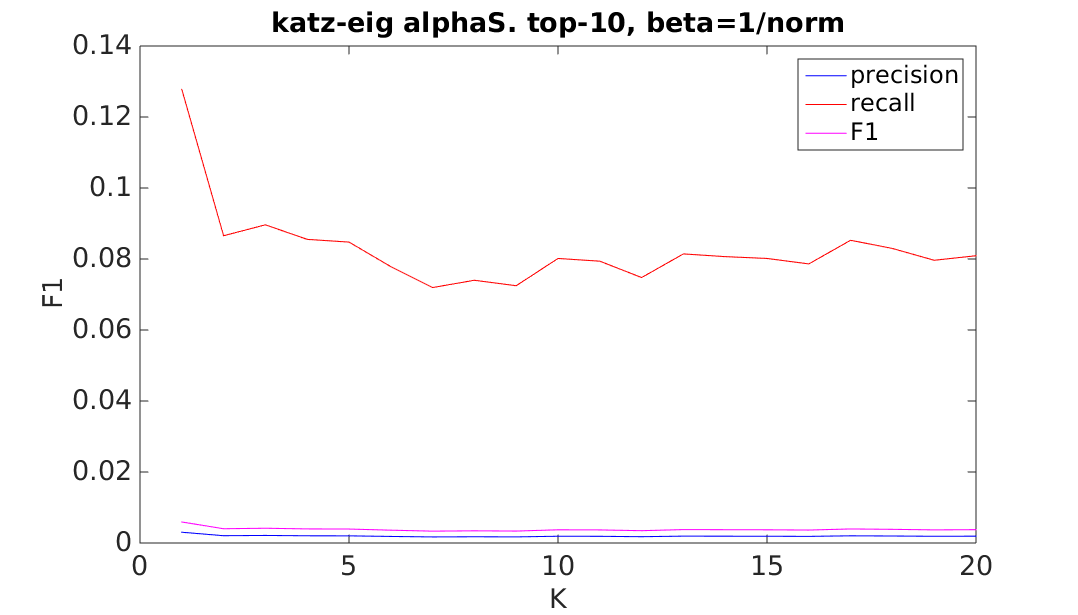
\includegraphics[width=\linewidth]{fig/katzeig_k/alphaS_katzeig_K.png}
    \captionof{figure}{\textit{alphaS} $K_{m} = 13$}
\end{minipage}%
\begin{minipage}{.5\textwidth}
    \centering
    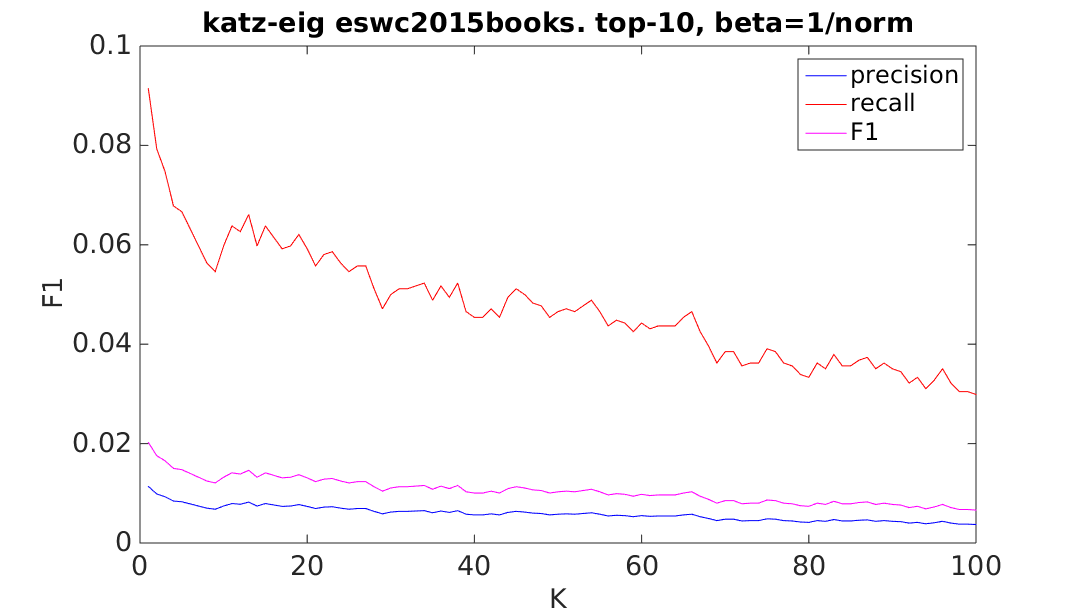
\includegraphics[width=\linewidth]{fig/katzeig_k/eswc2015books_katzeig_K.png}
    \captionof{figure}{\textit{eswc2015books} $K_{m} = 1$}
\end{minipage}
\end{figure}

\begin{figure}[h!]
\centering
\begin{minipage}{.5\textwidth}
    \centering
    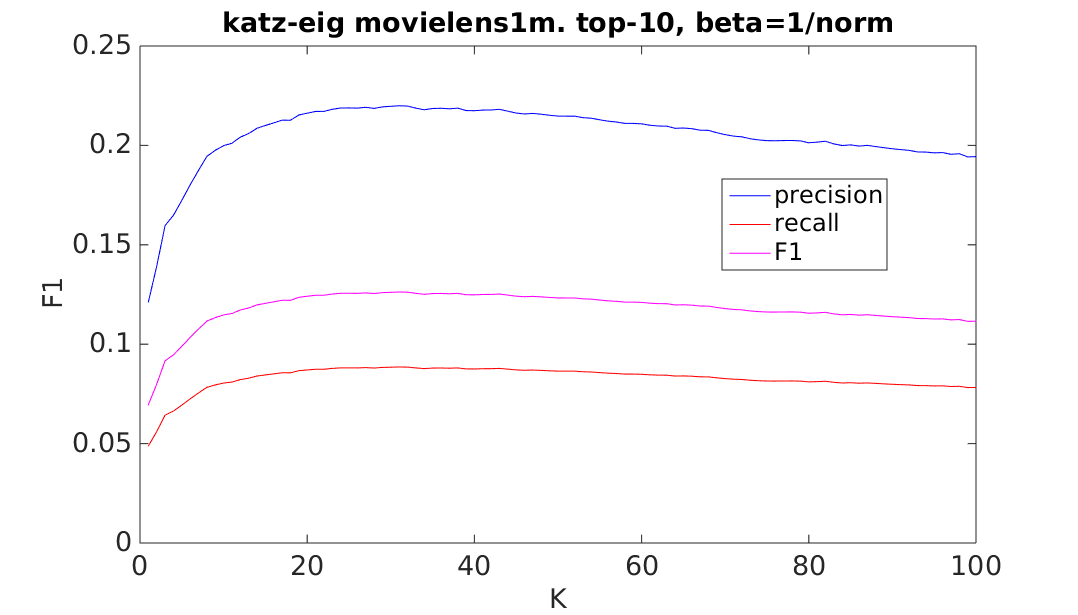
\includegraphics[width=\linewidth]{fig/katzeig_k/movielens_katzeig_K.png}
    \captionof{figure}{\textit{movielens1m} $K_{m} = 31$}
\end{minipage}%
\begin{minipage}{.5\textwidth}
    \centering
    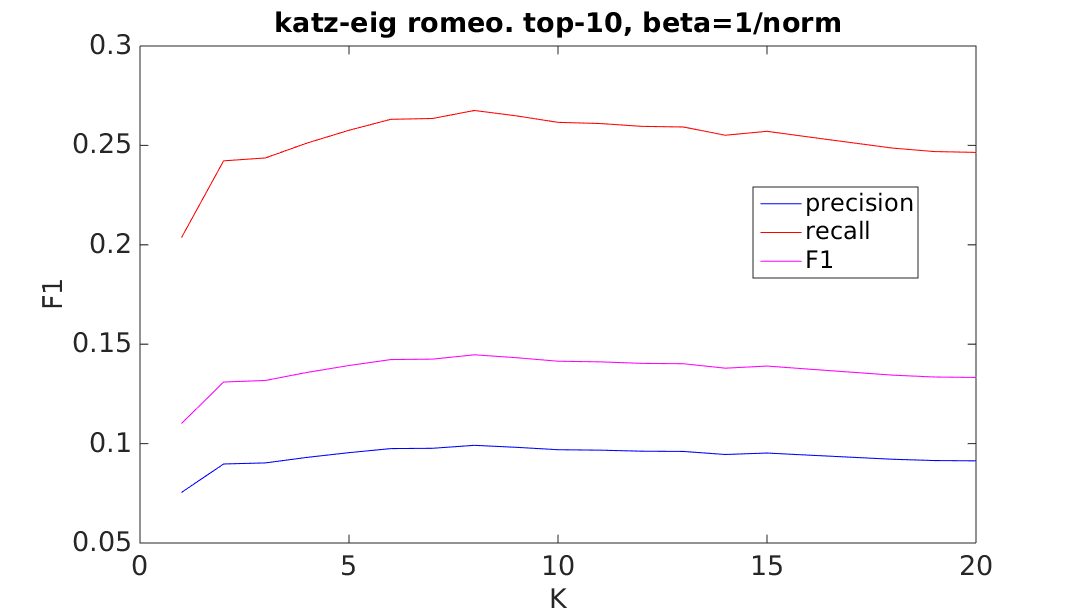
\includegraphics[width=\linewidth]{fig/katzeig_k/romeo_katzeig_K.png}
    \captionof{figure}{\textit{romeo} $K_{m} = 8$}
\end{minipage}
\end{figure}

\FloatBarrier

The function space with respect to $K$ is fairly smooth if not entirely convex. \textit{eswc2015books} is an outlier with a low optimal value $K = 1$ and many local optima. The other datasets display more smooth functions, but there are clear local optima with both \textit{alphaS} and \textit{romeo}.

